\documentclass[border=3mm]{standalone}

\usepackage{tikz}

\begin{document}
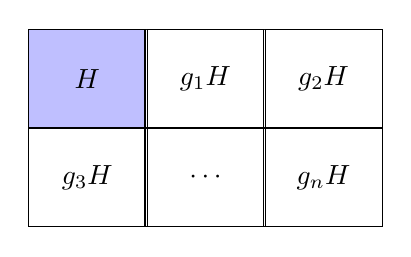
\begin{tikzpicture}
		\node[rectangle,minimum width=1.5cm,minimum height=1.25cm,fill=blue!25,inner sep=0pt](1) {$H$};
		\node[rectangle,minimum width=1.5cm,minimum height=1.25cm,right of=1,node distance=1.5cm](2) {$g_1H$};
		\node[rectangle,minimum width=1.5cm,minimum height=1.25cm,right of=2,node distance=1.5cm](3) {$g_2H$};
		\node[rectangle,minimum width=1.5cm,minimum height=1.25cm,below of=1,node distance=1.25cm](4) {$g_3H$};
		\node[rectangle,minimum width=1.5cm,minimum height=1.25cm,right of=4,node distance=1.5cm](5) {$\cdots$};
		\node[rectangle,minimum width=1.5cm,minimum height=1.25cm,right of=5,node distance=1.5cm](5) {$g_nH$};
		\draw (-0.75,0.625) -- (3.75,0.625) -- (3.75,-1.875) -- (-0.75,-1.875)-- cycle;
		\draw[double] (0.75,0.625) -- (0.75,-1.875);
		\draw[double] (2.25,0.625) -- (2.25,-1.875);
		\draw (-0.75,-0.625) -- (3.75,-0.625);
	\end{tikzpicture}
\end{document}
